\section{The particle zoo and experiments}

The quark model and the symmetry classification of hadrons did not arise from
abstract reasoning alone; they were forced upon physicists by an accumulating body
of experimental data. Before the ordering schemes of Chapter~3 can be appreciated,
it is worth retracing how the hadrons themselves were found, how their defining
quantum numbers were measured, and why their sheer number eventually demanded a
substructure. This chapter follows that historical and experimental thread, from the
earliest cosmic-ray detectors to the accelerator experiments that populated the
``particle zoo''.

\subsection{Early detectors and cosmic ray experiments}

At the beginning of the twentieth century the constituents of matter appeared to be
few and well understood. The electron had been identified in 1897, the proton was
established around 1920, the photon emerged from the work on the photoelectric and
Compton effects between 1905 and 1923, and the neutron was discovered in 1932.
With these building blocks a great deal could be explained: the chemical elements
and their periodic regularities, the structure of atoms, the existence of isotopes,
and the three classical types of radioactivity ($\alpha$, $\beta$ and $\gamma$).
Yet this apparent completeness was soon overturned by a steady stream of new
particles, most of which were first seen not in the laboratory but in the cosmic
radiation \cite[Ch.~2]{Amsler2018}.

The principal tool of this early period was the photographic, or nuclear, emulsion.
A charged particle traversing the emulsion loses energy by ionization and leaves a
latent track that becomes visible after development. Since the rate of energy loss
scales with the square of the particle's charge, $Z^2$, the grain density along a
track encodes information about the traversing particle. To intercept the primary
cosmic radiation before it was degraded in the atmosphere, emulsion stacks were
flown on balloons or exposed on mountain tops; the cosmic radiation itself had been
discovered by Hess in 1912 through electroscope measurements at altitude.

\begin{figure}[htbp]
    \centering
    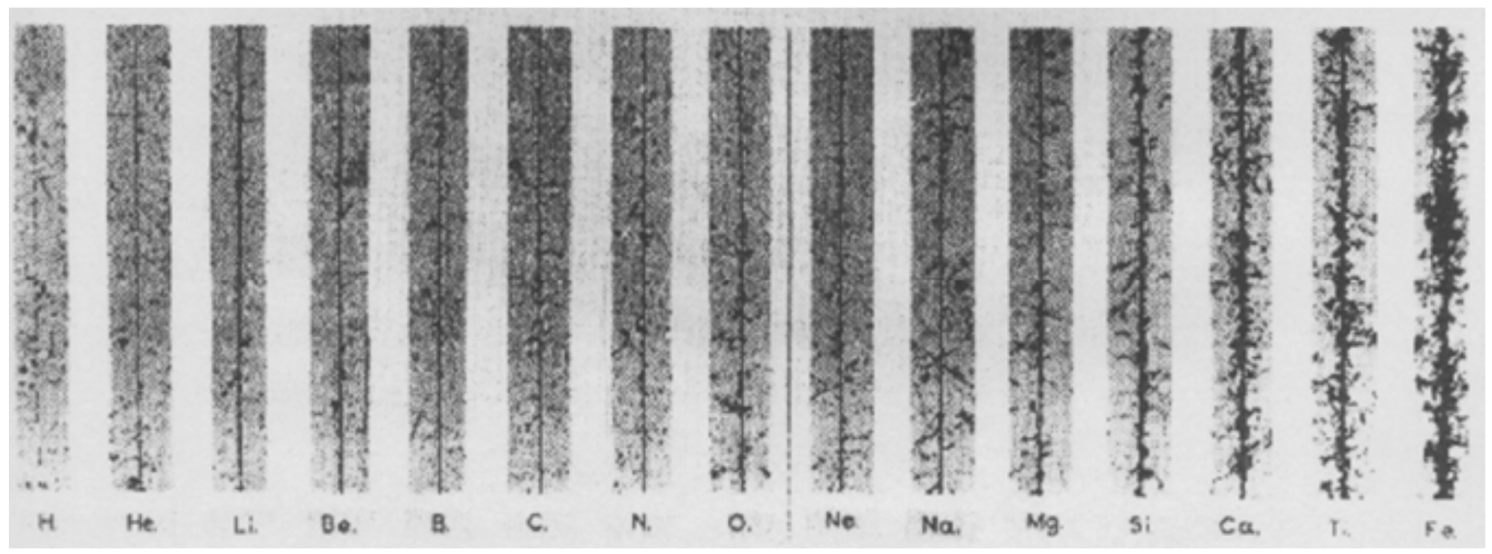
\includegraphics[width=0.75\linewidth]{Figures/EmulsionZ2.png}
    \caption{Nuclear emulsion tracks of cosmic-ray nuclei (H, He, Li, ... Fe), illustrating that the ionization density grows with $Z^2$. Adapted from the lecture slides (week 16, "Nuclear emulsion")}
    \label{fig:emulsionZ}
\end{figure}

The quantitative description of this ionization loss is given by the Bethe--Bloch
formula, which for a heavy charged particle (not an electron) reads, in the form
quoted in the lecture,
\begin{equation}
    \left\langle -\frac{dE}{dx} \right\rangle
    \;\approx\;
    K z^2 \frac{Z}{A} \frac{1}{\beta^2}
    \left[
        \frac{1}{2} \ln \frac{2 m_e c^2 \beta^2 \gamma^2 W_{\max}}{I^2} - \beta^2
    \right],
    \label{eq:bethe_bloch}
\end{equation}
where $z$ is the charge number of the incident particle, $Z$ and $A$ characterise
the absorber, $I$ is its mean excitation energy, $W_{\max}$ is the maximum energy
transferable to an atomic electron in a single collision, $K$ is a constant, and
$\beta = p/E$, $\gamma = E/M$ as usual. The energy loss falls steeply at low
velocity, passes through a broad minimum (the regime of minimum-ionizing
particles), and rises only logarithmically thereafter. Because a slow particle loses
energy ever more rapidly as it decelerates, the deposition is sharply peaked just
before the particle stops, a feature exploited in hadron tumor therapy. A
measurement of $dE/dx$ together with the momentum therefore separates particle
species, since at fixed momentum lighter particles are faster and ionize less than
heavier ones \cite[Ch.~2]{Amsler2018}.

\begin{figure}[htbp]
    \centering
    \begin{subfigure}[b]{0.45\textwidth}
        \centering
        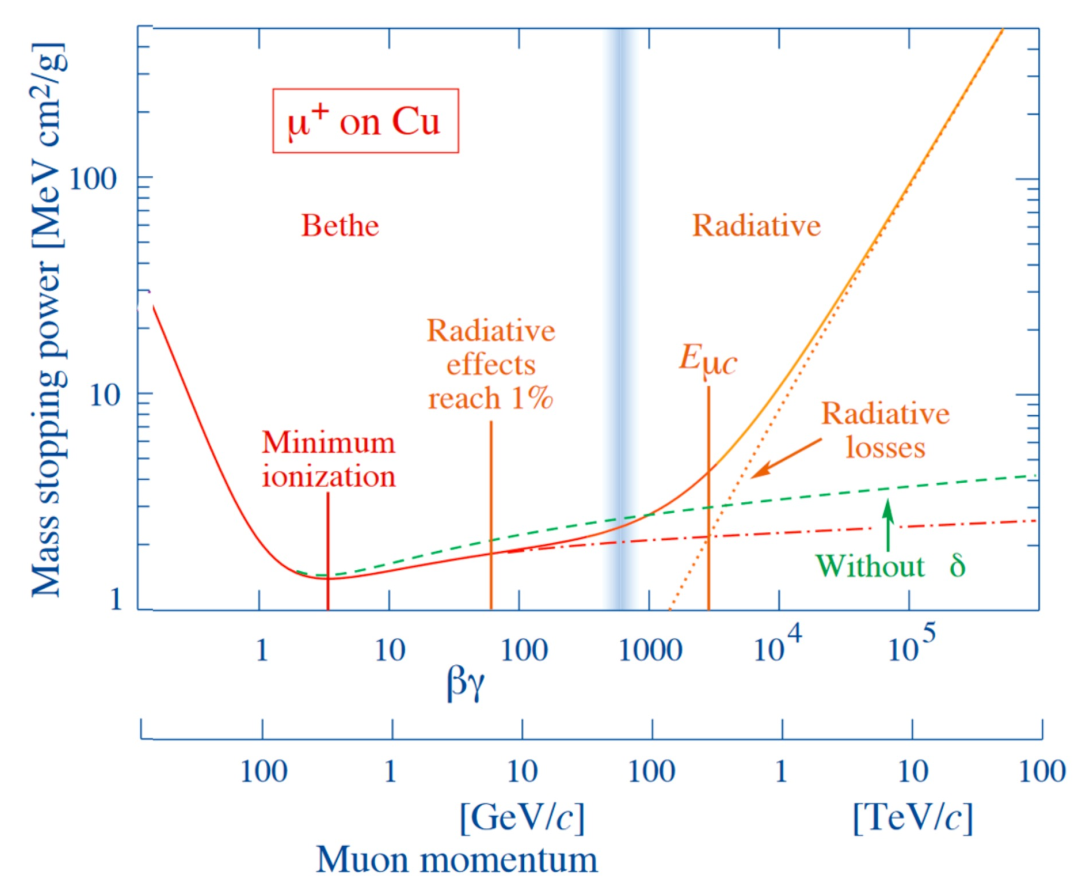
\includegraphics[width=\textwidth]{Figures/StoppingPower.png}
        \caption{Mass stopping power -dE/dx vs. beta-gamma for mu+ on Cu, showing the Bethe region, the minimum, and radiative losses at high energy}
        \label{fig:sub-first}
    \end{subfigure}
    \hfill
    \begin{subfigure}[b]{0.45\textwidth}
        \centering
        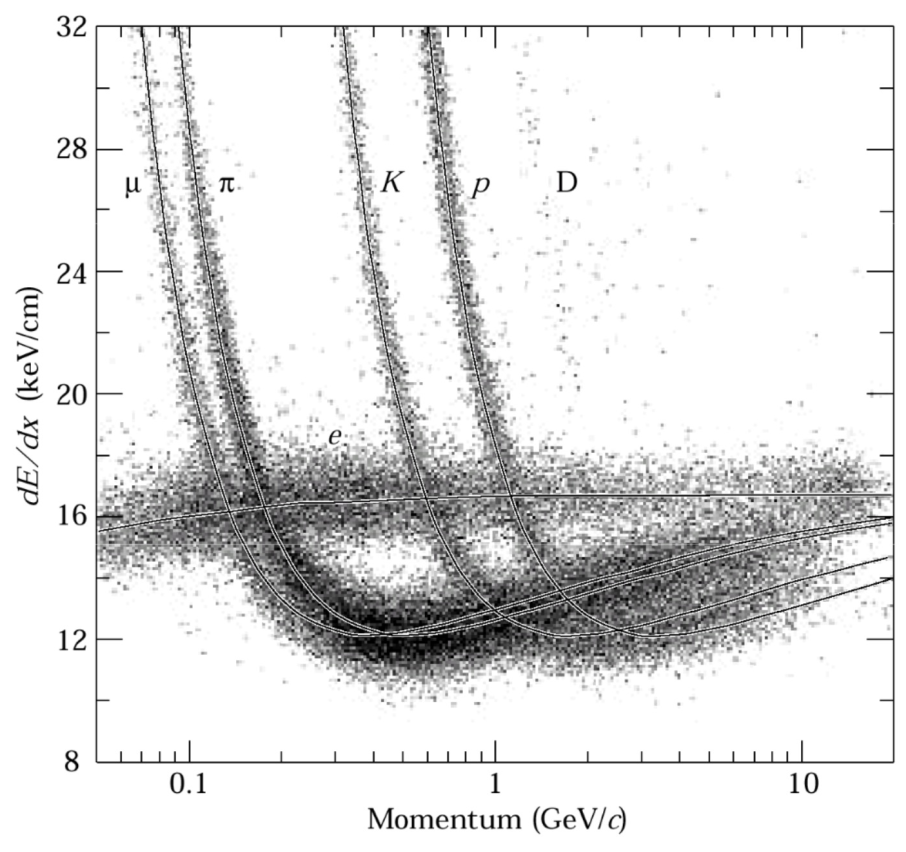
\includegraphics[width=\textwidth]{Figures/EnergyLoss.png}
        \caption{Measured dE/dx vs. momentum showing the separated mu, pi, K, p, D bands.}
        \label{fig:sub-second}
    \end{subfigure}
\end{figure}

The decisive cosmic-ray discovery for hadron physics was that of the charged pion.
A short-range mediator of the nuclear force had been postulated by Yukawa in 1935;
relating the range of the interaction, $R \sim 1\;\mathrm{fm}$, to the Compton
wavelength of the exchanged quantum yields a mass of order $200\,m_e$, that is
roughly $m_\pi \sim 200\;\mathrm{MeV}$ \cite[Ch.~2]{Amsler2018}. A particle found
in the cosmic radiation by Neddermeyer and Anderson in 1936 was at first taken to be
this quantum, but its failure to be absorbed by light nuclei showed it to be a
distinct, weakly interacting particle---the muon. The genuine Yukawa particle, the
charged pion with mass $m_\pi = 139.6\;\mathrm{MeV}$, was identified in 1947 by
Lattes, Occhialini and Powell using emulsions exposed at high altitude. The
characteristic decay sequence
\begin{equation}
    \pi^+ \;\to\; \mu^+ \;\to\; e^+
    \label{eq:pi_mu_e}
\end{equation}
was read directly from the emulsion: the constant range of the muon emerging from
the stopped pion signals the two-body decay $\pi^+ \to \mu^+ \nu_\mu$, the heavy
ionization near the ends of the pion and muon tracks marks their points of arrest,
and the faint track of the fast positron together with the Coulomb scattering of the
muon completes the identification \cite[Ch.~2]{Amsler2018}.

\subsection{The bubble chamber}

Emulsions provided exquisite spatial resolution but recorded events
indiscriminately and were laborious to scan. The bubble chamber, introduced in the
1950s, offered a controllable and repeatable alternative. Its active medium is a
liquid, often hydrogen, held just above its boiling point in a superheated state. A
charged particle crossing the liquid ionizes it along its path, and these ions act as
nucleation centers; a rapid decompression of the liquid then triggers boiling
precisely along the trajectory, so that a string of bubbles marks the track and can be
photographed. When the chamber sits in a magnetic field the trajectories curve, and
the sign and momentum of each particle follow from the sense and radius of
curvature. As in the emulsion, the bubble density along a track measures the
ionization and so contributes to particle identification through the combination of
curvature and ionization density. The principal limitation of the technique is its
speed: the compression cycle limits the repetition rate to about one expansion per
second or less \cite[Ch.~2]{Amsler2018}.

\begin{figure}[htbp]
    \centering
    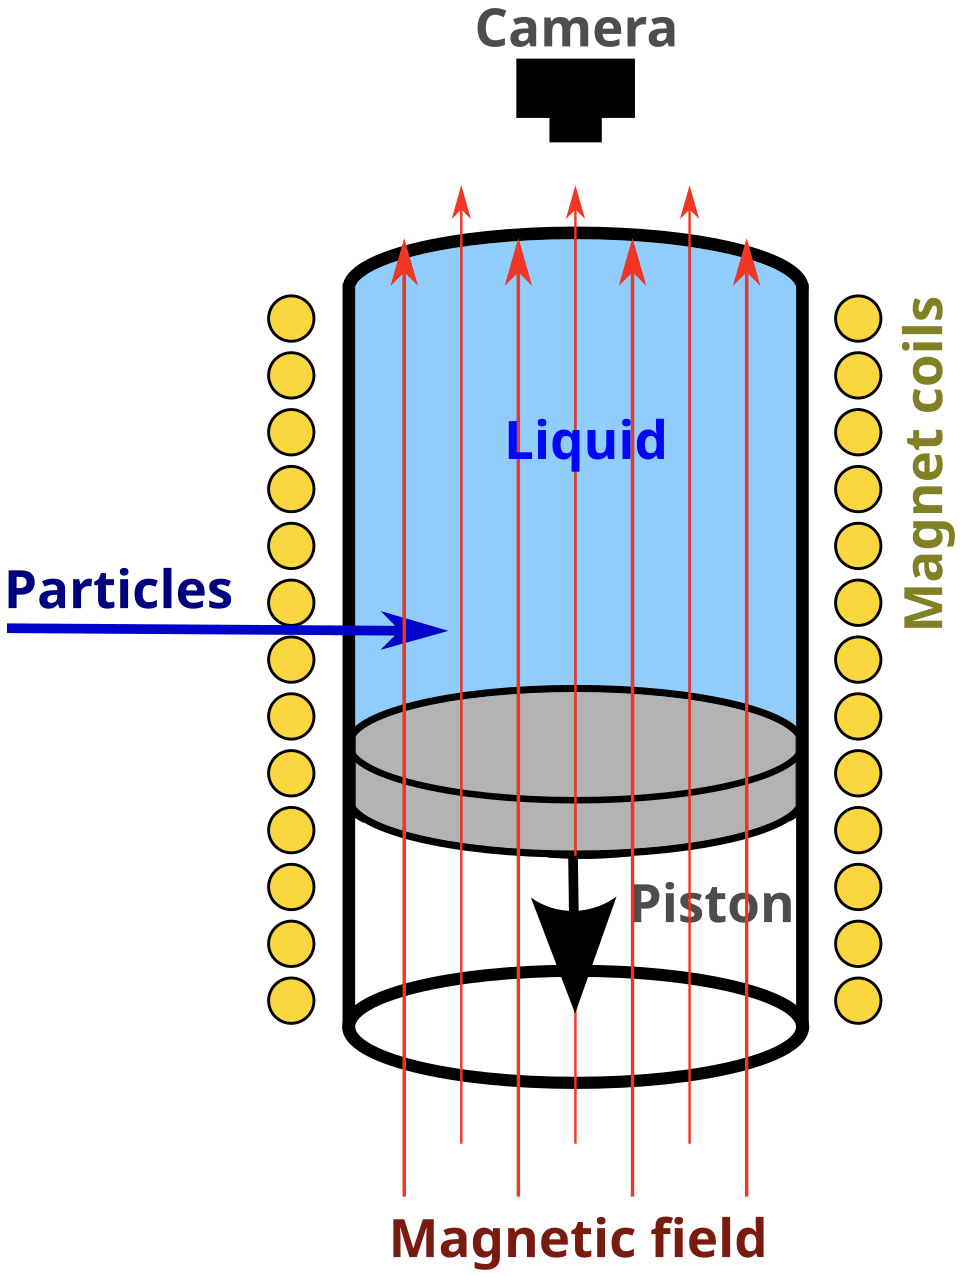
\includegraphics[width=0.5\linewidth]{Figures/BubbleChamber.png}
    \caption{Schematic of a bubble chamber: superheated liquid volume, incoming particle beam, piston for decompression, magnet coils producing the field, and an overhead camera.}
    \label{fig:bubblechamber}
\end{figure}

Such chambers were eventually built on a large scale. The Big European Bubble
Chamber (BEBC) at CERN, operated from the early 1970s, is a representative example;
analyses of its photographs continued into the 1990s. The hydrogen bubble chamber
became the workhorse instrument with which the strange baryons and the
$\Omega^-$ were established, as discussed in the next subsection.

\subsection{Hadron discovery at accelerators}

In the early 1950s particle accelerators became energetic enough to manufacture in
the laboratory the particles that had previously been glimpsed only in cosmic rays.
The Cosmotron at Brookhaven, for instance, accelerated protons to about
$3\;\mathrm{GeV}$, from which secondary pion beams of around $1.9\;\mathrm{GeV}$
could be derived. The defining experimental observation in these experiments was
the \emph{pairwise} production of the new ``strange'' particles: they were created
copiously, and always two at a time, in strong-interaction collisions, yet decayed
only slowly. This dichotomy was understood through a new additive quantum number,
strangeness $S$, conserved by the strong interaction that produces the particles but
violated by the weak interaction through which they decay---hence their description
as being produced in hadronic interactions but decaying weakly into hadrons
\cite[Ch.~2]{Amsler2018}.

The bubble-chamber and emulsion photographs of the period record a now-classic
catalogue of strange-particle production and decay. Neutral kaons were seen to
decay into pion pairs,
\begin{equation}
    K^0 \;\to\; \pi^+ \pi^- ,
\end{equation}
antiproton beams produced hyperon--antihyperon pairs such as
$\bar{p}p \to \bar{\Lambda}\Lambda$, and the charged and cascade hyperons revealed
themselves through their characteristic decay chains,
\begin{equation}
    \Sigma^+ \;\to\; p\,\pi^0 ,
    \qquad
    \Xi^- \;\to\; \Lambda \pi^- \;\to\; (p\,\pi^-)\,\pi^- .
\end{equation}
The cascade signature of the $\Xi^-$, decaying first to a $\Lambda$ and a pion and
then to a proton and a further pion, was particularly compelling evidence for a
hyperon carrying two units of strangeness. Later, neutrino beams---again analysed
in BEBC---extended this programme to weak production processes and to the charmed
hadrons \cite[Ch.~13]{Amsler2018}.

%% FIGURE SUGGESTION: Bubble-chamber or emulsion event displays of strange-particle
%% production, e.g. associated production of K and hyperons, with the decay chains
%% K0 -> pi+ pi-, ppbar -> Lambda Lambdabar, Sigma+ -> p pi0, and
%% Xi- -> Lambda pi- -> (p pi-) pi-. Adapted from the lecture slides (week 16,
%% "Discovery of hadrons") and Amsler (2018) Ch.~13.

\begin{figure}[htbp]
    \centering
    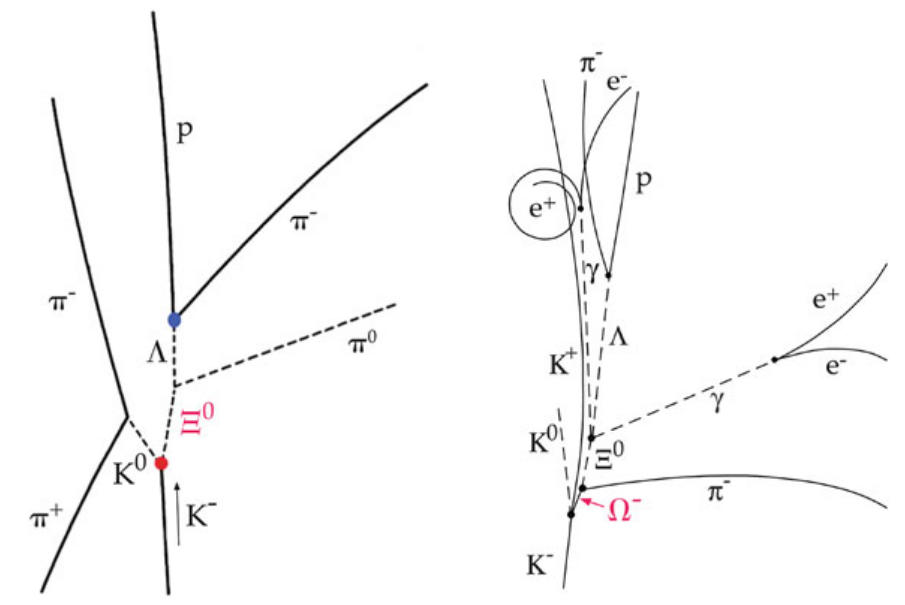
\includegraphics[width=0.75\linewidth]{Figures/BubbleChamberHyperonOmega.png}
    \caption{Bubble-chamber or emulsion event displays of strange-particle production, e.g. associated production of K and hyperons, with the decay chains $K_0 \rightarrow \pi^+ \pi^-$, $p \bar{p} \rightarrow \Lambda \bar{\Lambda}$, $\Sigma^+ -> p \pi_0$, and $\Xi^- -> \Lambda \pi^- \rightarrow (p \pi^-) \pi^-$}
    \label{fig:bublehyperon}
\end{figure}



\subsection{Determining particle properties}

Identifying a new hadron means measuring the set of characteristic quantum numbers
that distinguish it: its mass, its spin $J$, its parity $P$, its isospin $I$, its
baryon number $B$ and its strangeness $S$. Of these, the mass is the most directly
accessible. For a particle that decays into a set of measured daughters, or that is
produced in a reaction whose other products are measured, the mass follows from
energy--momentum conservation applied to the four-momenta. Writing the
four-momentum of particle $i$ as $P_i = (E_i, p_{x,i}, p_{y,i}, p_{z,i})$, the
invariant mass of a system reconstructed from two measured particles is
\begin{equation}
    m \;=\; \sqrt{\left(P_1 + P_2\right)^2},
    \label{eq:invariant_mass}
\end{equation}
where the square denotes the Lorentz-invariant scalar product of the total
four-momentum with itself. Because expression~\eqref{eq:invariant_mass} is a
Lorentz invariant, the same value is obtained in any reference frame, which is what
makes it the natural observable for identifying a resonance as a peak in a mass
spectrum \cite[Ch.~2]{Amsler2018}. The remaining quantum numbers $J$, $P$, $I$,
$B$ and $S$ are not read off a single track but are inferred from production and
decay patterns, angular distributions, and conservation laws; the determination of
the pion spin treated below is the prototypical example, and the strangeness
assignments follow from the associated-production rule of the previous subsection.

\subsection{Reconstructing masses: invariant mass and missing mass}

In practice two complementary strategies are used to evaluate
expression~\eqref{eq:invariant_mass}, depending on which particles a given detector
can measure. The first is a \emph{direct} reconstruction, in which all decay
products are detected and their four-momenta summed. A meson decaying to two
photons illustrates the method: in a calorimeter that records the energies and
directions of both photons, the squared invariant mass is simply
\begin{equation}
    m_{\gamma\gamma}^2 \;=\; \left(P_{\gamma,1} + P_{\gamma,2}\right)^2 ,
    \label{eq:direct_mass}
\end{equation}
and a histogram of $m_{\gamma\gamma}$ over many events shows peaks at the
$\pi^0$ and $\eta$ masses. The Crystal Barrel experiment at ELSA, for example,
isolates the $\eta \to \gamma\gamma$ signal in this way.

The second strategy is the \emph{missing-mass} method, used when the particle of
interest is not itself detected but recoils against a measured system. In the
photoproduction reaction $\gamma p \to \eta p$ with $\eta \to \gamma\gamma$, the
recoiling proton is measured in a tracking detector while the beam and target
four-momenta are known; the mass recoiling against the proton is then
\begin{equation}
    m_{\gamma\gamma}^2
    \;=\;
    \left(P_{\gamma,\mathrm{beam}} + P_{p,\mathrm{target}} - P_{p,\mathrm{meas}}\right)^2 .
    \label{eq:missing_mass}
\end{equation}
A peak in this missing mass at the $\eta$ mass confirms the reaction without any
direct observation of the meson's decay products. The CLAS experiment at Jefferson
Lab exemplifies this approach. The two methods are complementary: the direct method
demands full detection of the decay products, whereas the missing-mass method
trades that requirement for precise knowledge of the initial state and of the
recoiling system \cite[Ch.~2]{Amsler2018}.

%% FIGURE SUGGESTION: Side-by-side mass spectra illustrating the two methods.
%% (left) Direct gamma-gamma invariant mass spectrum (Crystal Barrel at ELSA) with
%% pi0 and eta peaks; (right) missing-mass spectrum (CLAS at Jefferson Lab) for
%% gamma p -> eta p showing pi0, eta, omega/rho and eta' peaks. Adapted from the
%% lecture slides (week 16, "Reconstructing meson masses -- an example").

\subsection{Determination of the pion spin}

The spin of the charged pion provides a clean illustration of how a quantum number
can be extracted from cross-section measurements alone, without any knowledge of
the underlying dynamics. The argument compares a reaction with its time reverse at
the same centre-of-mass energy,
\begin{equation}
    A: \quad pp \to \pi^+ d ,
    \qquad\qquad
    B: \quad \pi^+ d \to pp ,
    \label{eq:pi_spin_reactions}
\end{equation}
and rests on the principle of detailed balance. In a scattering process the
transition rate is given by Fermi's golden rule,
\begin{equation}
    W \;=\; \frac{2\pi}{\hbar}\,\lvert \mathcal{M}_{fi} \rvert^2 \rho_f ,
    \label{eq:golden_rule}
\end{equation}
where $\mathcal{M}_{fi}$ is the invariant transition amplitude connecting the
initial state $\lvert i \rangle$ to the final state $\lvert f \rangle$ and
$\rho_f$ is the density of final states. For the strong interaction
$\mathcal{M}_{fi}$ cannot be computed from first principles, and this is precisely
what the comparison of $A$ and $B$ is designed to circumvent
\cite[Ch.~2]{Amsler2018}.

Expressing the cross section of a two-body reaction
$a + b \to c + d$ through the squared amplitude and the appropriate spin
multiplicities and phase-space factors gives, in the notation of the lecture,
\begin{equation}
    \sigma(a + b \to c + d)
    \;=\;
    \lvert \mathcal{M}_{fi} \rvert^2
    \,\frac{(2 s_c + 1)(2 s_d + 1)}{v_i v_f}\, p_f^2 .
    \label{eq:sigma_general}
\end{equation}
Applying this to the two reactions in~\eqref{eq:pi_spin_reactions} with the proton
spin $s_p = \tfrac{1}{2}$ and the deuteron spin $s_d = 1$, and using the fact that
the strong interaction is invariant under both time reversal and space inversion---so
that the squared amplitudes are equal at the same centre-of-mass energy,
$\lvert \mathcal{M}_{fi} \rvert^2 = \lvert \mathcal{M}_{if} \rvert^2$---the unknown
amplitude cancels in the ratio. Care must be taken with the spin averaging:
reaction $A$ has initial spin multiplicity $(2 s_p + 1)^2 = 4$, of which only the
identical-particle factor $\tfrac{1}{2}$ survives in the final state, while reaction
$B$ carries the factor $(2 s_d + 1)(2 s_\pi + 1) = 3(2 s_\pi + 1)$. The result is
\begin{equation}
    \frac{\sigma(pp \to \pi^+ d)}{\sigma(\pi^+ d \to pp)}
    \;=\;
    \frac{3}{2}\,(2 s_\pi + 1)\,\frac{p_\pi^2}{p_p^2} ,
    \label{eq:pi_spin_ratio}
\end{equation}
where $p_\pi$ and $p_p$ are the centre-of-mass momenta of the pion and the proton
respectively \cite[Ch.~2]{Amsler2018}.

The right-hand side of~\eqref{eq:pi_spin_ratio} depends only on measurable momenta
and on the single unknown $s_\pi$. The first measurements, from Cartwright and
collaborators around 1950--1951 and from Durbin and collaborators in 1951---the
latter using a proton beam of kinetic energy $T_p = 340\;\mathrm{MeV}$ at the
Berkeley cyclotron---yielded a ratio consistent only with $s_\pi = 0$. The pion is
therefore a spinless particle, in keeping with its later interpretation as a
ground-state $q\bar{q}$ meson \cite[Ch.~2]{Amsler2018}.

%% FIGURE SUGGESTION: Comparison of the measured differential cross sections for
%% pi+ d -> pp and pp -> pi+ d (or the energy dependence of the two cross sections),
%% overlaid with the predictions for s_pi = 0 and s_pi = 1, demonstrating the clear
%% preference for s_pi = 0. Adapted from the lecture slides (week 16,
%% "Determination of the pion-spin") and the data of Cartwright et al. and
%% Durbin et al.

\subsection{Ordering the particle zoo: towards the quark model}

By the late 1950s the experimental programmes described above had produced an
embarrassment of riches. So many strongly interacting particles had been found that
they could no longer all be regarded as elementary, a situation captured in Fermi's
quip that had he been able to remember the names of all the particles he would have
become a botanist, and in Lamb's wry suggestion that the discovery of a new particle
ought to be punished rather than rewarded. The proliferation---the so-called
``particle zoo''---demanded an organising principle analogous to the periodic table
of the chemical elements, and the very existence of such a regularity would point,
as it had for atoms, to an underlying substructure \cite[Ch.~1]{Amsler2018}.

The resolution came from the use of symmetry and group theory. Gell-Mann and, in a
related development, Ne'eman recognised around 1961--1964 that the known hadrons
fall naturally into multiplets of the approximate flavour symmetry group
$\mathrm{SU}(3)_f$, a scheme that Gell-Mann named the Eightfold Way
\cite[Ch.~2]{HalzenMartin1984}. The fundamental representation of $\mathrm{SU}(3)$
is three-dimensional, and Gell-Mann and, independently, Zweig proposed in 1964 that
these three basis states correspond to physical (at the time hypothetical)
constituents, the quarks $u$, $d$ and $s$. Gell-Mann drew the name from a line in
James Joyce's \textit{Finnegans Wake}, ``Three quarks for Muster Mark''. In this
picture the mesons, which carry integer spin, are quark--antiquark combinations
$q\bar{q}$, while the baryons, which carry half-integer spin, are three-quark
combinations $qqq$ \cite[Ch.~1]{Amsler2018}.

%% FIGURE SUGGESTION: The lightest SU(3)_f weight diagrams: the pseudoscalar meson
%% nonet (qqbar) and the spin-1/2 baryon octet (qqq), plotted in the strangeness vs.
%% charge plane, with the original excerpt from Gell-Mann's 1964 "A Schematic Model
%% of Baryons and Mesons". Adapted from the lecture slides (week 16, "Order in the
%% zoo") and Amsler (2018) Ch.~7, Ch.~13.

The classifying power of the scheme was striking: the lightest pseudoscalar and
vector mesons group into octets and singlets, and the lightest baryons into an octet
and a decuplet. Its most celebrated success was predictive rather than merely
descriptive. The pattern of the spin-$\tfrac{3}{2}$ baryon decuplet left a single
vacant position, a triply strange state, whose mass could be read off from the
equal spacing of the other members. The corresponding particle, the $\Omega^-$, was
duly observed in a bubble chamber at Brookhaven in 1964 with a mass close to the
predicted value, a confirmation that transformed the quark model from a bookkeeping
device into a description of genuine substructure \cite[Ch.~7]{Amsler2018}. The
group-theoretical machinery that underlies these multiplets---isospin, the
construction of $\mathrm{SU}(N)$ representations, and the weight diagrams---is the
subject of the following chapter.